\documentclass{standalone}
\usepackage{tikz}
\usetikzlibrary{patterns, positioning}


\begin{document}
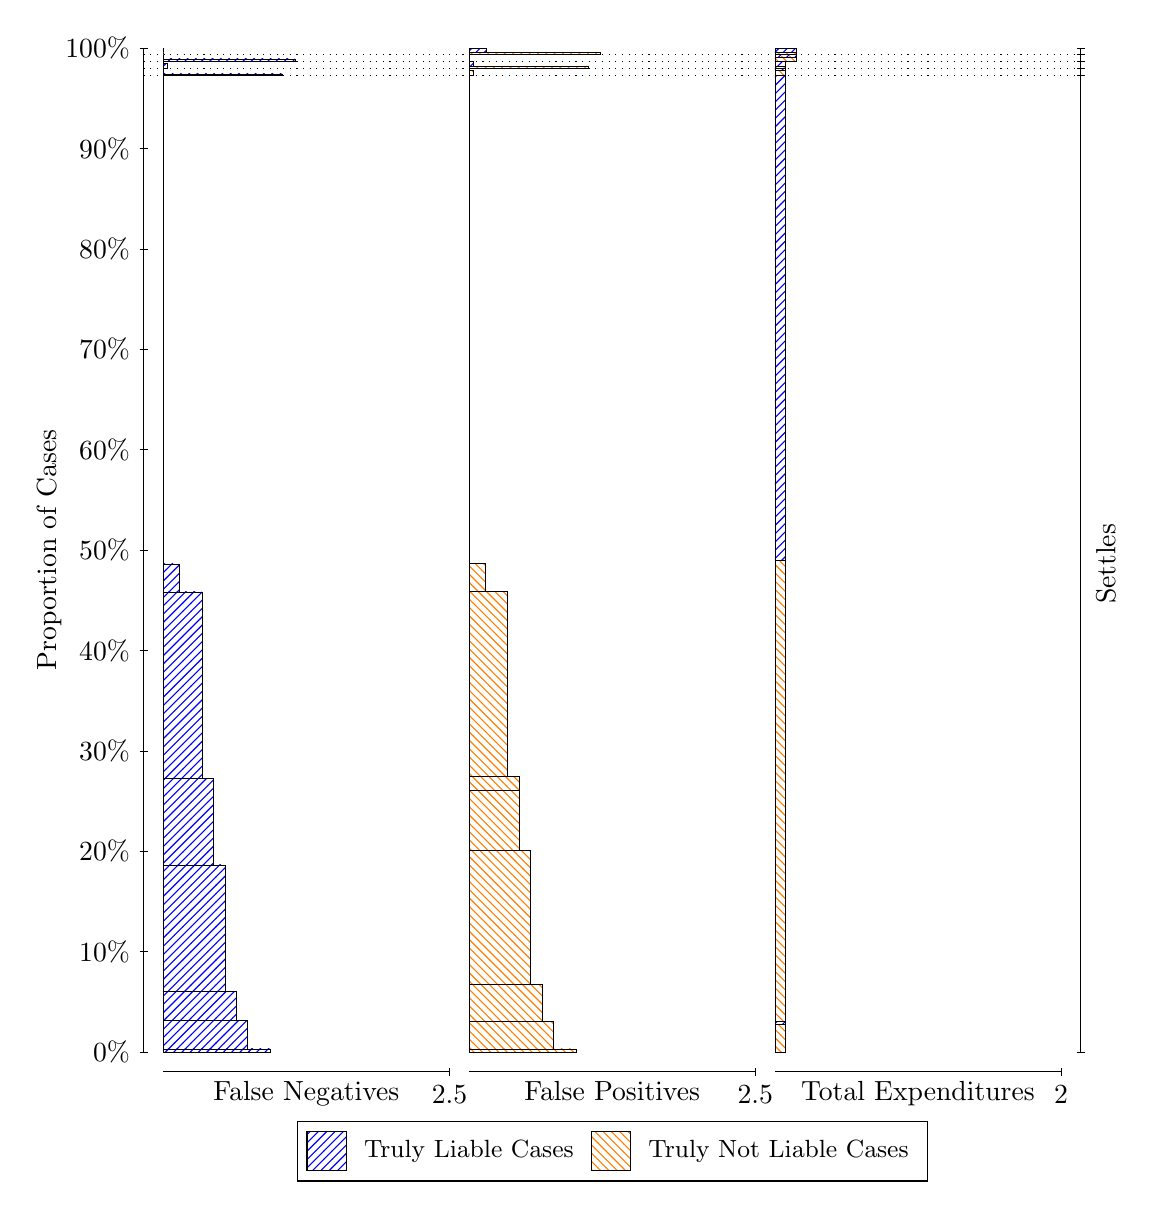
\begin{tikzpicture}
\draw[black, very thin] (1.5,1.75) -- (1.5,14.5);
\node[rotate=90, text=black, anchor=center] at (0.3, 8.125) {Proportion of Cases};
\draw[black, very thin] (1.45,1.75) -- (1.55,1.75);
\node[text=black, anchor=east] at (1.45, 1.75) {0\%};
\draw[black, very thin] (1.45,3.025) -- (1.55,3.025);
\node[text=black, anchor=east] at (1.45, 3.025) {10\%};
\draw[black, very thin] (1.45,4.3) -- (1.55,4.3);
\node[text=black, anchor=east] at (1.45, 4.3) {20\%};
\draw[black, very thin] (1.45,5.575) -- (1.55,5.575);
\node[text=black, anchor=east] at (1.45, 5.575) {30\%};
\draw[black, very thin] (1.45,6.85) -- (1.55,6.85);
\node[text=black, anchor=east] at (1.45, 6.85) {40\%};
\draw[black, very thin] (1.45,8.125) -- (1.55,8.125);
\node[text=black, anchor=east] at (1.45, 8.125) {50\%};
\draw[black, very thin] (1.45,9.4) -- (1.55,9.4);
\node[text=black, anchor=east] at (1.45, 9.4) {60\%};
\draw[black, very thin] (1.45,10.675) -- (1.55,10.675);
\node[text=black, anchor=east] at (1.45, 10.675) {70\%};
\draw[black, very thin] (1.45,11.95) -- (1.55,11.95);
\node[text=black, anchor=east] at (1.45, 11.95) {80\%};
\draw[black, very thin] (1.45,13.225) -- (1.55,13.225);
\node[text=black, anchor=east] at (1.45, 13.225) {90\%};
\draw[black, very thin] (1.45,14.5) -- (1.55,14.5);
\node[text=black, anchor=east] at (1.45, 14.5) {100\%};

\draw[black, very thin] (13.4,1.75) -- (13.4,14.5);
\draw[black, very thin] (13.35,1.75) -- (13.45,1.75);
\node[anchor=west] at (13.35, 1.75) {};
\draw[black, very thin] (13.35,14.148) -- (13.45,14.148);
\node[anchor=west] at (13.35, 14.148) {};
\draw[black, very thin] (13.35,14.237) -- (13.45,14.237);
\node[anchor=west] at (13.35, 14.237) {};
\draw[black, very thin] (13.35,14.333) -- (13.45,14.333);
\node[anchor=west] at (13.35, 14.333) {};
\draw[black, very thin] (13.35,14.416) -- (13.45,14.416);
\node[anchor=west] at (13.35, 14.416) {};
\draw[black, very thin] (13.35,14.5) -- (13.45,14.5);
\node[anchor=west] at (13.35, 14.5) {};

\draw[black, very thin, pattern color=blue, pattern=north east lines] (1.75,1.75) rectangle (3.1125,1.7895);
\draw[black, very thin, pattern color=blue, pattern=north east lines] (1.75,1.7895) rectangle (2.8218,2.1518);
\draw[black, very thin, pattern color=blue, pattern=north east lines] (1.75,2.1518) rectangle (2.6765,2.5213);
\draw[black, very thin, pattern color=blue, pattern=north east lines] (1.75,2.5213) rectangle (2.5312,4.1254);
\draw[black, very thin, pattern color=blue, pattern=north east lines] (1.75,4.1254) rectangle (2.3858,5.2255);
\draw[black, very thin, pattern color=blue, pattern=north east lines] (1.75,5.2255) rectangle (2.2405,7.594);
\draw[black, very thin, pattern color=blue, pattern=north east lines] (1.75,7.594) rectangle (1.9498,7.9474);
\draw[black, very thin, pattern color=orange, pattern=north west lines] (1.75,7.9474) rectangle (1.75,14.148);
\draw[black, very thin, pattern color=blue, pattern=north east lines] (1.75,14.148) rectangle (3.2578,14.171);
\draw[black, very thin, pattern color=orange, pattern=north west lines] (1.75,14.171) rectangle (1.75,14.237);
\draw[black, very thin, pattern color=blue, pattern=north east lines] (1.75,14.237) rectangle (1.8045,14.307);
\draw[black, very thin, pattern color=orange, pattern=north west lines] (1.75,14.307) rectangle (1.75,14.333);
\draw[black, very thin, pattern color=blue, pattern=north east lines] (1.75,14.333) rectangle (3.4213,14.361);
\draw[black, very thin, pattern color=orange, pattern=north west lines] (1.75,14.361) rectangle (1.75,14.416);
\draw[black, very thin, pattern color=orange, pattern=north west lines] (1.75,14.416) rectangle (1.75,14.444);
\draw[black, very thin, pattern color=blue, pattern=north east lines] (1.75,14.444) rectangle (1.75,14.5);
\draw[black, very thin, pattern color=orange, pattern=north west lines] (5.6333,1.75) rectangle (6.9958,1.7895);
\draw[black, very thin, pattern color=orange, pattern=north west lines] (5.6333,1.7895) rectangle (6.7052,2.14);
\draw[black, very thin, pattern color=orange, pattern=north west lines] (5.6333,2.14) rectangle (6.5598,2.6043);
\draw[black, very thin, pattern color=orange, pattern=north west lines] (5.6333,2.6043) rectangle (6.4145,4.3124);
\draw[black, very thin, pattern color=orange, pattern=north west lines] (5.6333,4.3124) rectangle (6.2692,5.0708);
\draw[black, very thin, pattern color=orange, pattern=north west lines] (5.6333,5.0708) rectangle (6.2692,5.2534);
\draw[black, very thin, pattern color=orange, pattern=north west lines] (5.6333,5.2534) rectangle (6.1238,7.5971);
\draw[black, very thin, pattern color=orange, pattern=north west lines] (5.6333,7.5971) rectangle (5.8332,7.9506);
\draw[black, very thin, pattern color=blue, pattern=north east lines] (5.6333,7.9506) rectangle (5.6333,14.148);
\draw[black, very thin, pattern color=orange, pattern=north west lines] (5.6333,14.148) rectangle (5.6878,14.214);
\draw[black, very thin, pattern color=blue, pattern=north east lines] (5.6333,14.214) rectangle (5.6333,14.237);
\draw[black, very thin, pattern color=orange, pattern=north west lines] (5.6333,14.237) rectangle (7.1412,14.262);
\draw[black, very thin, pattern color=blue, pattern=north east lines] (5.6333,14.262) rectangle (5.6878,14.333);
\draw[black, very thin, pattern color=orange, pattern=north west lines] (5.6333,14.333) rectangle (5.6333,14.387);
\draw[black, very thin, pattern color=blue, pattern=north east lines] (5.6333,14.387) rectangle (5.6333,14.416);
\draw[black, very thin, pattern color=orange, pattern=north west lines] (5.6333,14.416) rectangle (7.3047,14.444);
\draw[black, very thin, pattern color=blue, pattern=north east lines] (5.6333,14.444) rectangle (5.8513,14.5);
\draw[black, very thin, pattern color=orange, pattern=north west lines] (9.5167,1.75) rectangle (9.6529,2.1034);
\draw[black, very thin, pattern color=blue, pattern=north east lines] (9.5167,2.1034) rectangle (9.6529,2.1429);
\draw[black, very thin, pattern color=orange, pattern=north west lines] (9.5167,2.1429) rectangle (9.6529,7.99);
\draw[black, very thin, pattern color=blue, pattern=north east lines] (9.5167,7.99) rectangle (9.6529,14.148);
\draw[black, very thin, pattern color=orange, pattern=north west lines] (9.5167,14.148) rectangle (9.6529,14.214);
\draw[black, very thin, pattern color=blue, pattern=north east lines] (9.5167,14.214) rectangle (9.6529,14.237);
\draw[black, very thin, pattern color=orange, pattern=north west lines] (9.5167,14.237) rectangle (9.6529,14.262);
\draw[black, very thin, pattern color=blue, pattern=north east lines] (9.5167,14.262) rectangle (9.6529,14.333);
\draw[black, very thin, pattern color=orange, pattern=north west lines] (9.5167,14.333) rectangle (9.7892,14.387);
\draw[black, very thin, pattern color=blue, pattern=north east lines] (9.5167,14.387) rectangle (9.7892,14.416);
\draw[black, very thin, pattern color=orange, pattern=north west lines] (9.5167,14.416) rectangle (9.7892,14.444);
\draw[black, very thin, pattern color=blue, pattern=north east lines] (9.5167,14.444) rectangle (9.7892,14.5);
\draw[black, dotted] (1.5,14.148) -- (13.4,14.148);
\draw[black, dotted] (1.5,14.237) -- (13.4,14.237);
\draw[black, dotted] (1.5,14.333) -- (13.4,14.333);
\draw[black, dotted] (1.5,14.416) -- (13.4,14.416);
\draw[black, very thin] (1.75,1.5) -- (5.3833,1.5);
\node[text=black, anchor=north] at (3.5667, 1.5) {False Negatives};
\draw[black, very thin] (5.3833,1.45) -- (5.3833,1.55);
\node[text=black, anchor=north] at (5.3833, 1.45) {2.5};

\draw[black, very thin] (5.6333,1.5) -- (9.2667,1.5);
\node[text=black, anchor=north] at (7.45, 1.5) {False Positives};
\draw[black, very thin] (9.2667,1.45) -- (9.2667,1.55);
\node[text=black, anchor=north] at (9.2667, 1.45) {2.5};

\draw[black, very thin] (9.5167,1.5) -- (13.15,1.5);
\node[text=black, anchor=north] at (11.333, 1.5) {Total Expenditures};
\draw[black, very thin] (13.15,1.45) -- (13.15,1.55);
\node[text=black, anchor=north] at (13.15, 1.45) {2};

\node[text=black, centered, rotate=90] at (13.72, 7.949) {Settles};





\draw (7.449999999999999,1.5) node[draw=none] (baseCoordinate) {};
\begin{scope}[align=center]
        \matrix[scale=0.5, draw=black, below=0.5cm of baseCoordinate, nodes={draw}, column sep=0.1cm]{
            \node[rectangle, draw, minimum width=0.5cm, minimum height=0.5cm, pattern color=blue, pattern=north east lines] {}; &
            \node[draw=none, font=\small, text=black] (B) {Truly Liable Cases}; &
            \node[rectangle, draw, minimum width=0.5cm, minimum height=0.5cm, pattern color=orange, pattern=north west lines] {}; &
            \node[draw=none, font=\small, text=black] (B) {Truly Not Liable Cases}; \\
            };
\end{scope}

\end{tikzpicture}
\end{document}